\documentclass[11pt]{article}

% Use the following to compile
% mkdir tmp
% pdflatex -aux-directory=tmp -output-directory=tmp --shell-escape notes.tex

% Package use definitions
\usepackage[margin=1in]{geometry}
\usepackage{fancyhdr}
\usepackage[parfill]{parskip}
\usepackage{graphicx}
\usepackage{comment}
\usepackage[outputdir=tmp]{minted}
\usepackage[dvipsnames]{xcolor}
\usepackage{listings}
\usepackage[hidelinks]{hyperref}
\usepackage{amsmath}
\usepackage{amsfonts}
\usepackage{amssymb}
\usepackage{tcolorbox}
\usepackage{tabu}
\usepackage{upgreek}
\usepackage[ruled,vlined]{algorithm2e}
\usepackage[nottoc]{tocbibind}
\usepackage{natbib}

\setlength{\parindent}{11pt}
\setlength{\parskip}{0pt}

% Header and footer setup
\pagestyle{fancy} \rhead{\today} \lhead{Book} \renewcommand{\headrulewidth}{1pt}
\renewcommand{\footrulewidth}{1pt}

% Image directory specification
\graphicspath{ {./images/} }

% Settings minted option for the entire document
\definecolor{LightGray}{rgb}{0.9, 0.9, 0.9}
\setminted{frame=lines,framesep=2mm,bgcolor=LightGray,linenos,
  fontsize=\footnotesize, baselinestretch=1.2}

% Start of document
\begin{document}

% Title page and table of contents setup
\begin{titlepage}
  \begin{center}
    \vspace*{1cm} \Huge \textbf{SCALA Project}\\
    %% \vspace*{1\baselineskip} Notes\\
    \vspace*{2\baselineskip} \large
    \vfill \normalsize \textbf{Dorian Mignon}\\ \textbf{Christopher Diamana
      Lutete}\\ \textbf{Alexis Morton}\\ \textbf{Jose A. Henriquez Roa}\\
    \vspace*{2\baselineskip} \today \rhead{\today}
    \newpage
    \normalsize \tableofcontents
    \newpage
  \end{center}
\end{titlepage}

% Document Body:
\section{Preliminary questions}
\subsection{Question 1}
\paragraph{Question} What technical/business constraints should the data storage
component of the program architecture meet to fulfill the requirement described
by the customer in paragraph ``Statistics''?\\\\ As described by the ``Statistics''
section of the subject the storage component will be required to hold
peacemakers' reports as well as the peacewatchers' temporal series. We assume
the former to be some type of unstructured data (word documents or PDFs) while
the latter will most like be represented in a semi-structured data format (XML,
JSON, etc.). Additionally, it is specified that the estimate of a day's worth of
peacewatchers' reports will occupy around 200Gb, which on it's own greatly
influences the choice of type storage component. Finally with regards to the CAP
theorem, It is also safe to assume that since this is a police force related
task the storage component will most likely rather benefit from being
``available'' and ``partition tolerant'' and trade-off consistency by having data be
propagated at night or some other time when there is less activity.\par Thus, we
have the following requirement:
\begin{enumerate}
\item AP type
\item able to natively store different data types
\item able to manage store large amounts of data
\end{enumerate}
\paragraph{Question} So what kind of component(s) (listed in the lecture) will
the architecture need?\\\\
Out of the ones presented during the lectures, the storage component type that
is fits all of the previous points is the \textit{Data Lake}.
\subsection{Question 2}
\paragraph{Question} What business constraint should the architecture meet to
fulfill the requirement describe in the paragraph ``Alert''?\\\\ The ``Alert''
section mostly describes constraints on the type of distributed processing. This
section brings forth the necessity of an ``fast'' alert system.\par The two
distributed processing types presented during the lecture were Batch processing
and Stream processing. As implied by the name batch processing treats the data
only on a given schedule or when a given quota is met. Stream processing on the
other hand treats the data in a continuous matter. It also allows for multiple
data buses for when the data needs to be redirected to multiple (stream)
consumers.\par Seen as peacewatcher's are deployable field units meant for
gathering data it is best to offload any type of alert directed data-processing
to a separate dedicated and more secure unit. The task of this new unit would
then consist of processing incoming data from the peacewatchers and forward
alerts to the peacemakers when need be. This new unit essentially defines
another data (stream) consumer in addition to our previous data storage
component. Finally, we note from the peacewatchers' description that the
generated per-minute reports are mostly consisting of a small number of integers
and strings making the entire reports relatively small in size, and thus a good
fit for Stream processing.\par In summary, we note the new requirement for
\textit{Stream processing} and a dedicated \textit{Alert Processing Unit}.
\subsection{Question 3}
\paragraph{Question} What mistake(s) from Peaceland can explains the failed
attempt?\\\\
The sentence: ``\textit{not been able to set up a scalable program that can
  handle the load}'' leads to believe that a mistake was made in the choice of
the storage component, where one not natively fit for large amounts of data was
chosen. The mistake could also have been in the choice of the distributed
processing type, where the team could have chosen batch processing, which would
inevitably result a large accumulation of data if processing was setup to be
done on a ill-adapted schedule.
\subsection{Question 4} Peaceland has likely forgotten some technical
information in the report sent by the drone. In the future this information
could help Peaceland make its peacewatchers much more efficient. Which
information?\\\\ From what is gathered by the "Drone Description" section,
regarding the recorded words heard in the vicinity of the peacewatcher, being
able to discern from which citizen the recorded words originated from will most
likely be use for updating their designated "peace score". Seen as the drone is
already able to detect the name of the citazen through facial recognition and
hear the words spoken in it's surrounding, this was most likely a forgotten
feature.
\section{Project}
For a solution to this problem we consider the following minimal architecture:\\
\begin{figure}[H]
  \centering
  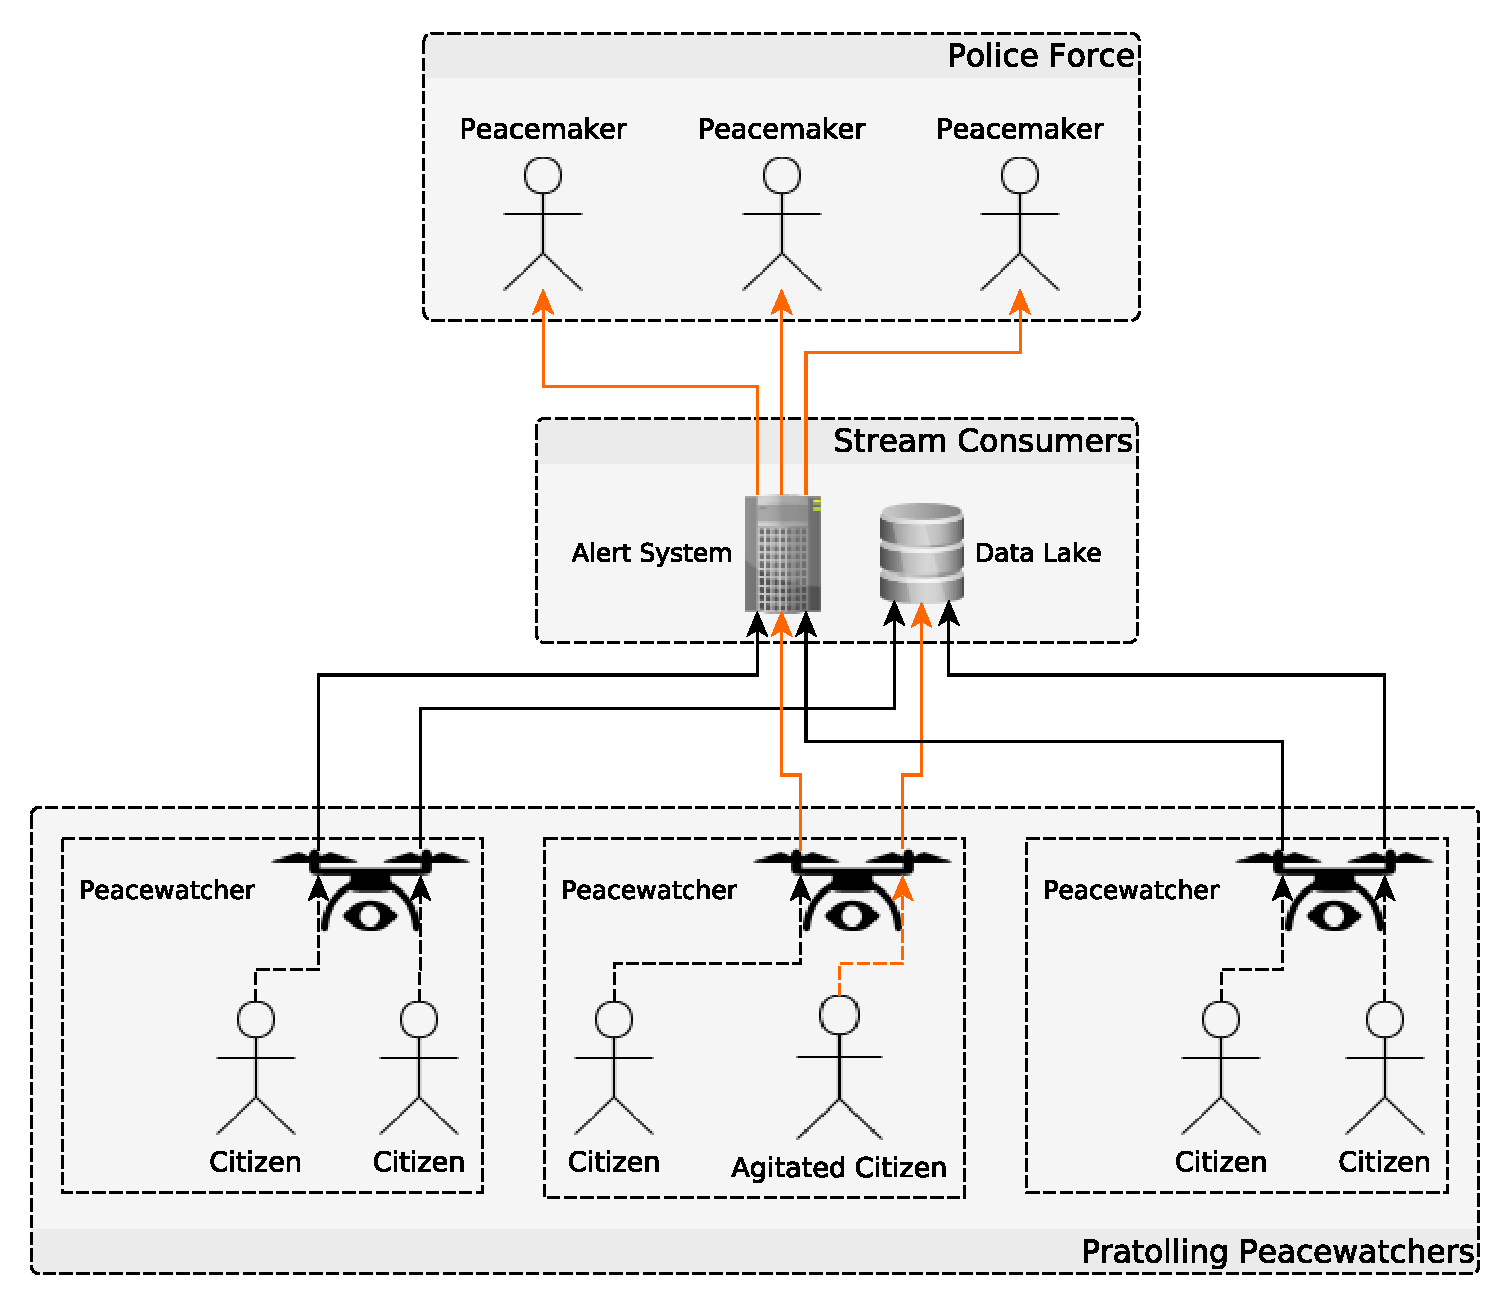
\includegraphics[scale=0.4]{image/minimal.pdf}
  \caption{Proposed minimal architecture}
\end{figure}
For the previously stated reasons we consider a Data Lake as the storage
component as well as a stream processing alert system. Both of which constitute
two stream consumers. Were the alert system analyses the data and the Data Lake
simply stores it for later use. With this architecture peacewatchers send
collected data to both the alert system and the storage component. These two
could be situated behind own private network if needed. Upon receiving a report
from an agitated citizen the alert system simply forwards this one to the
peacemakers as shown in the diagram.\par Depending on the size of the region in
which to implemented the program, this one could possible benefit from a more
modular variation of the previous architecture. This new one is described by the
following diagram:
\begin{figure}[H]
  \centering
  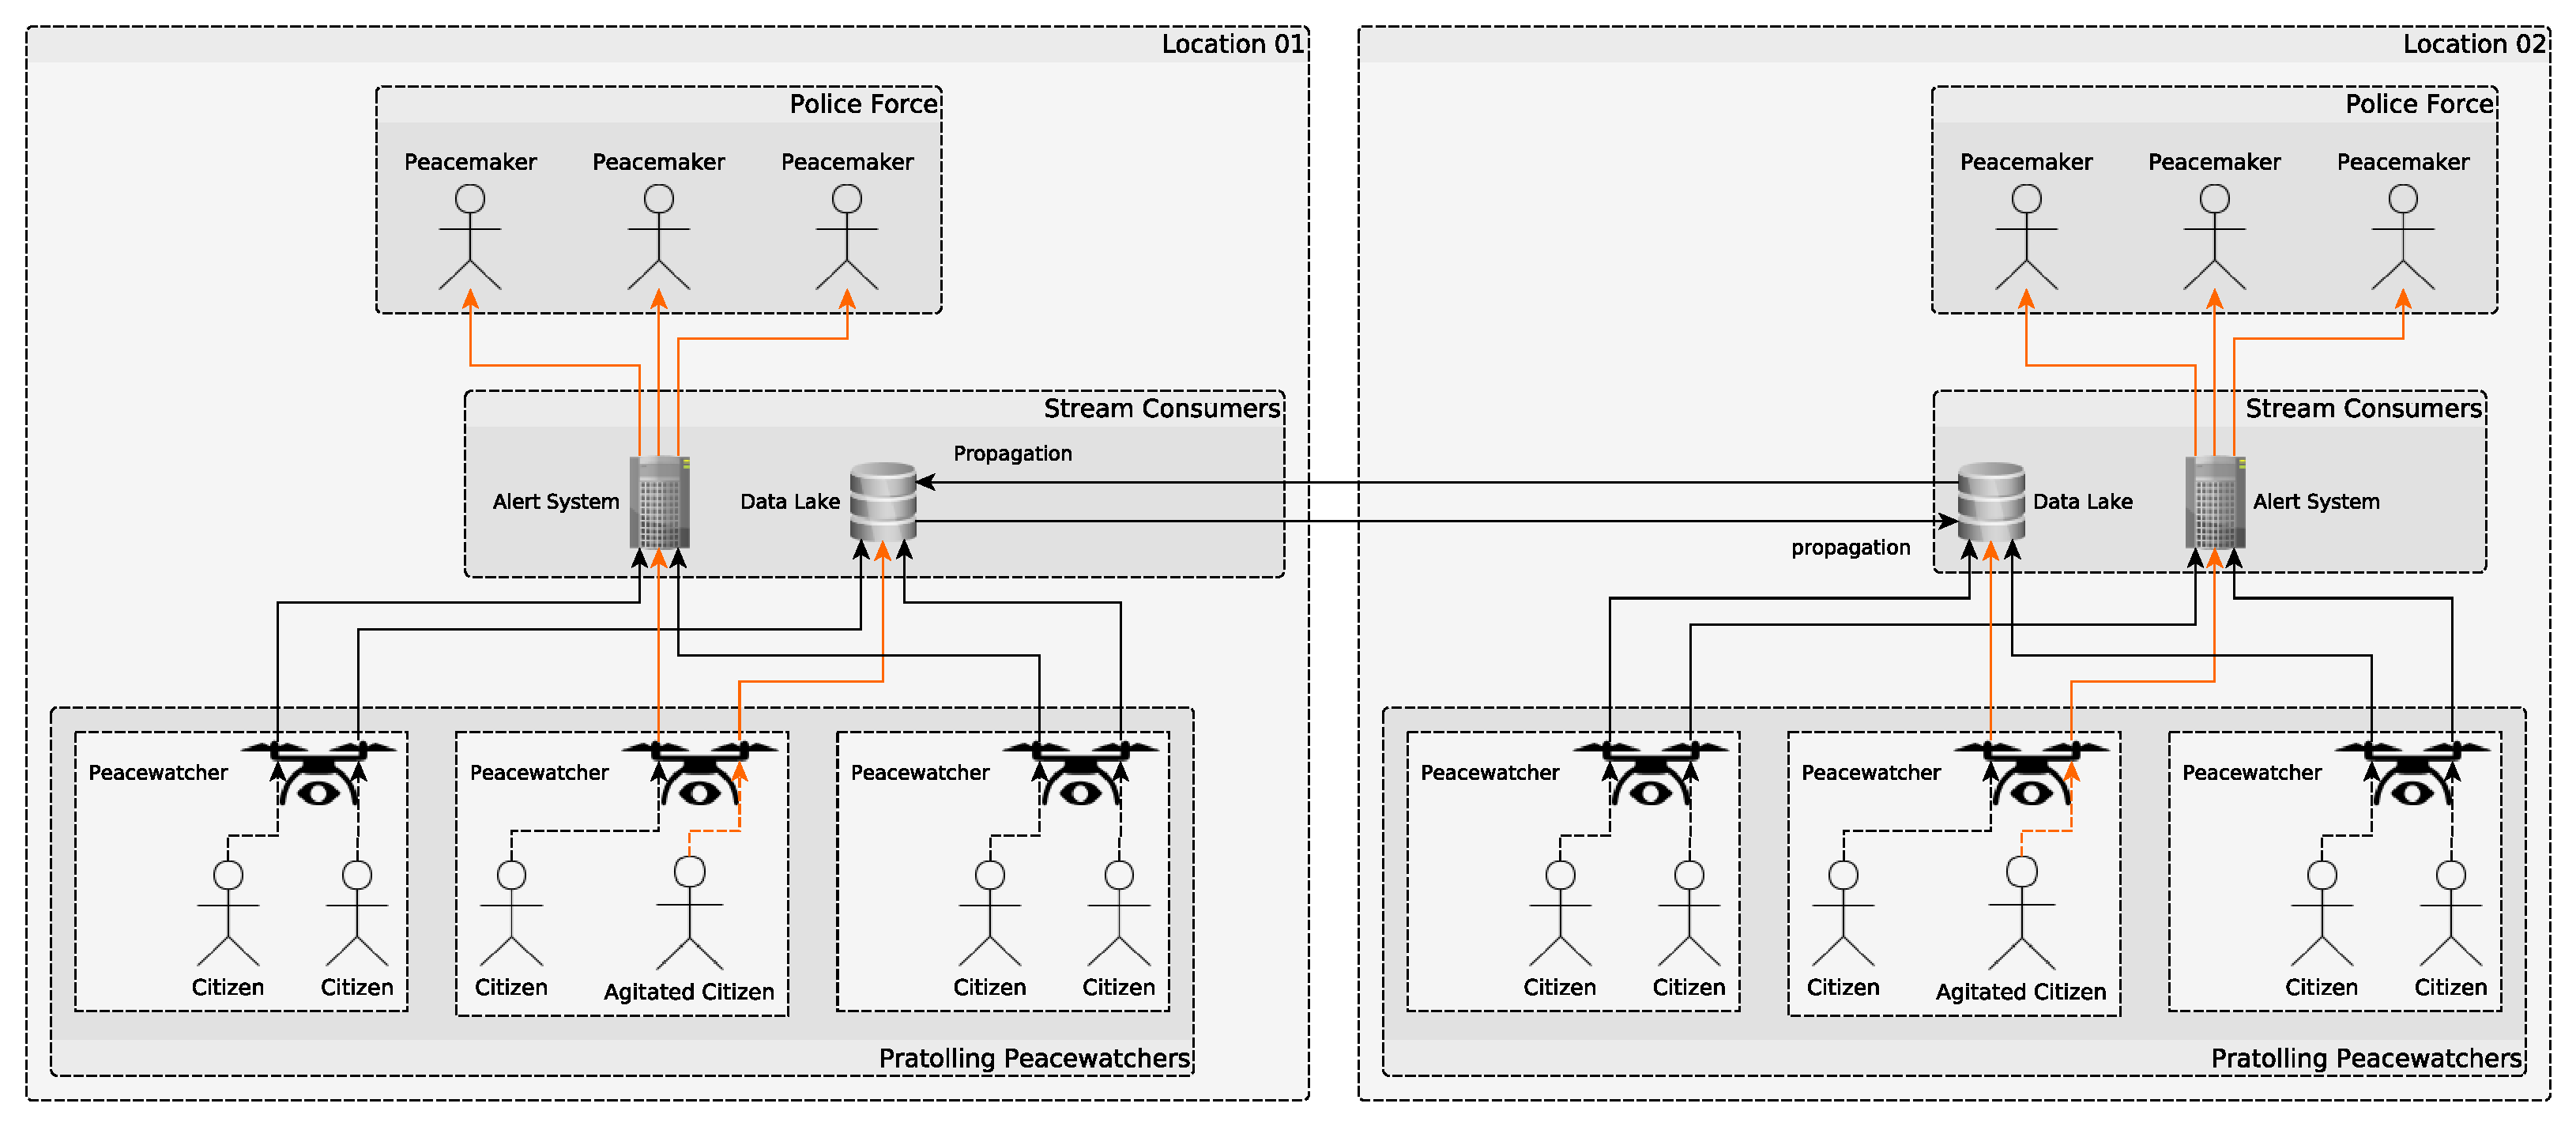
\includegraphics[scale=0.3]{image/multiple.pdf}
  \caption{Proposed modular architecture}
\end{figure}
If the program were to be implemented over a large region there would be no
need for all peacemakers to be notified of all agitated citizen in all regions,
but rather only the ones is the same nearby regions. This would be solved by
this new architecture. To keep data up to data on all regions an additional
"propagation" stream between storage components is setup. With this ones data
could be replicated during the night when there is less police activity. An
additional benefit of this one is that, through the more modular, aspect it
increases fault tolerance and adds robustness to the entire system. We also note
that depending on the cloud service provider the components themselves could be
split among smaller regions for seperate reasons which are not to be confused
with the previously stated ones.
\end{document}
